\documentclass[a4paper,english]{article}
%\usepackage[T1]{fontenc}		% la font bien
\usepackage[utf8]{inputenc}		% les accents
\usepackage[french]{babel}		% la langue
\usepackage{amsmath,amssymb,breqn}	% math
\usepackage{graphicx,color,import,float,subcaption}  % graph
\usepackage[usenames,dvipsnames]{xcolor}
\usepackage[margin=2.4cm]{geometry} % marges
\usepackage{multicol,multirow}	% tables
\usepackage{todonotes}			% penses-bêtes
\usepackage{wrapfig}			% figures sur le côté
\usepackage{hyperref}			% liens vers les figures et formules
\usepackage{lipsum, comment}

\renewcommand{\thesubfigure}{\roman{subfigure}} 
% Numérotation romaine des sous-figures pour éviter collision avec légende

\begin{document}

\title{Thinfilm}
\author{Jeanne Colbois \& Mario Geiger}
\date{\today}
\maketitle

\section{Matrice de transfert}

\begin{figure}[H]
	\centering
	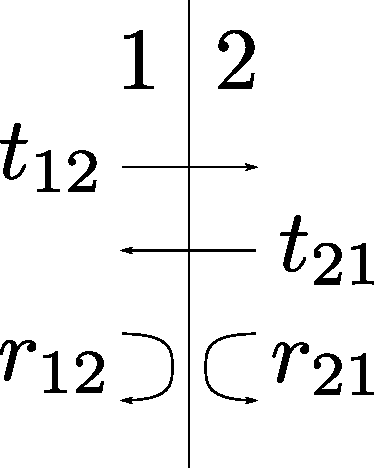
\includegraphics[height=3cm]{interface.pdf}
\end{figure}

$\rightarrow_1$ est la phase et amplitude de l'onde incidente depuis la gauche. $\leftarrow_1$ est la phase et amplitude de l'onde réfléchie vers la gauche. $\rightarrow_2$ est celle de l'onde transmise et finalement $\leftarrow_2$ est nul.

\begin{equation}
\left\{ \begin{array}{lll}
\rightarrow_2 = t_{12} \rightarrow_1 + r_{21} \leftarrow_2  &\Rightarrow &\rightarrow_1 = \frac{\rightarrow_2 - r_{21} \leftarrow_2}{t_{12}} \\
\leftarrow_1 = t_{21} \leftarrow_2 + r_{12} \rightarrow_1 &\Rightarrow &\leftarrow_1 = t_{21} \leftarrow_2 + r_{12} \frac{\rightarrow_2 - r_{21} \leftarrow_2}{t_{12}}
\end{array}\right. 
\end{equation}

\begin{equation}\label{mtrans}
\begin{pmatrix}\rightarrow \\ \leftarrow \end{pmatrix}_1 = 
\frac{1}{t_{12}}\begin{pmatrix} 1 & -r_{21} \\ r_{12} & t_{12}t_{21} - r_{12}r_{21} \end{pmatrix} 
\begin{pmatrix}\rightarrow \\ \leftarrow\end{pmatrix}_2
\end{equation}


















\section{Fresnel}


\begin{figure}[H]
	\centering
	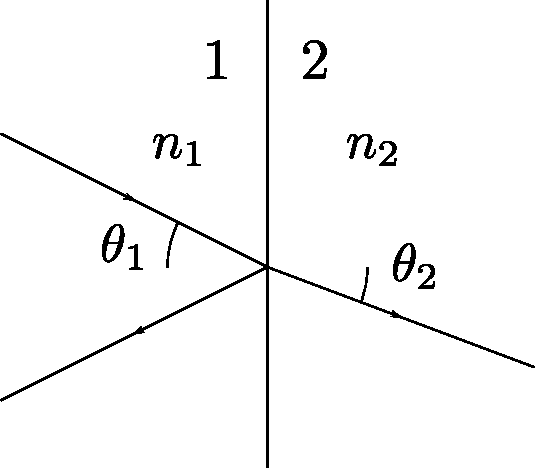
\includegraphics[height=3cm]{fresnel.pdf}
\end{figure}

\paragraph{Polarisation perpendiculaire}
\begin{equation}
\left\{ \begin{array}{l} 
r_s = r_{12} = \frac{n_1 \cos \theta_1 - n_2 \cos \theta_2}{n_1 \cos \theta_1 + n_2 \cos \theta_2} = \frac{\eta_1 - \eta_2}{\eta_1 + \eta_2} \\
t_s = t_{12} = \frac{2 n_1 \cos \theta_1}{n_1 \cos \theta_1 + n_2 \cos \theta_2} = \frac{2 \eta_1}{\eta_1 + \eta_2}
\end{array} \right.
\end{equation}
Avec $\eta = n \cos \theta$.

\paragraph{Polarisation parallèle}
\begin{equation}
\left\{ \begin{array}{l} 
r_p = r_{12} = \frac{n_1 \cos \theta_2 - n_2 \cos \theta_1}{n_2 \cos \theta_1 + n_1 \cos \theta_2} = \frac{\eta_1 - \eta_2}{\eta_1 + \eta_2} \\
t_p = t_{12} = \frac{2 n_1 \cos \theta_1}{n_2 \cos \theta_1 + n_1 \cos \theta_2} = \frac{2 n_1 / \cos \theta_2}{\eta_1 + \eta_2} = \frac{2 \frac{n_1}{n_2} \eta_2}{\eta_1 + \eta_2}
\end{array} \right.
\end{equation}
Avec $\eta = n / \cos \theta$.

















\section{Matrice de transfert de Fresnel}
\paragraph{Polarisation perpendiculaire}
\begin{dmath}\label{mfress}
\frac{1}{t_{12}}\begin{pmatrix} 1 & -r_{21} \\ r_{12} & t_{12}t_{21} - r_{12}r_{21} \end{pmatrix} = 
\frac{1}{2 \eta_1} \begin{pmatrix} \eta_1 + \eta_2 & \eta_1 - \eta_2 \\ \eta_1 - \eta_2 & \frac{2 \eta_1 2 \eta_2}{\eta_1 + \eta_2} - \frac{(\eta_1 - \eta_2)(\eta_2 - \eta_1)}{\eta_1 + \eta_2} \end{pmatrix} =
\frac{1}{2 \eta_1} \begin{pmatrix} \eta_1 + \eta_2 & \eta_1 - \eta_2 \\ \eta_1 - \eta_2 & \eta_1 + \eta_2 \end{pmatrix} = 
\frac{1}{2 \eta_1} \begin{pmatrix} \eta_1 & 1 \\ \eta_1 & -1 \end{pmatrix}\begin{pmatrix} 1 & 1 \\ \eta_2 & -\eta_2 \end{pmatrix}
\end{dmath}


\paragraph{Polarisation parallèle}
\begin{dmath}\label{mfresp}
\frac{1}{t_{12}}\begin{pmatrix} 1 & -r_{21} \\ r_{12} & t_{12}t_{21} - r_{12}r_{21} \end{pmatrix} = 
\frac{1}{2 \frac{n_1}{n_2} \eta_2} \begin{pmatrix} \eta_1 + \eta_2 & \eta_1 - \eta_2 \\ \eta_1 - \eta_2 & \frac{2 \frac{n_1}{n_2} \eta_2 2 \frac{n_2}{n_1} \eta_1}{\eta_1 + \eta_2} - \frac{(\eta_1 - \eta_2)(\eta_2 - \eta_1)}{\eta_1 + \eta_2} \end{pmatrix} =
\frac{1}{2 \frac{n_1}{n_2} \eta_2} \begin{pmatrix} \eta_1 + \eta_2 & \eta_1 - \eta_2 \\ \eta_1 - \eta_2 & \eta_1 + \eta_2 \end{pmatrix} =
\frac{1}{2 n_1} \begin{pmatrix} \eta_1 & 1 \\ \eta_1 & -1 \end{pmatrix} \frac{n_2}{\eta_2} \begin{pmatrix} 1 & 1 \\ \eta_2 & -\eta_2 \end{pmatrix}
\end{dmath}














\section{Matrice de transfert de propagation}
\begin{figure}[H]
	\centering
	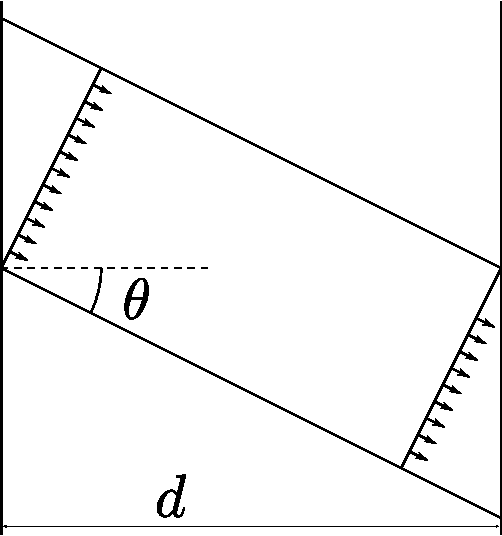
\includegraphics[height=3cm]{propagation.pdf}
\end{figure}

On a $t_{12} = t_{21} = \psi$ et aucune réflexion.
\begin{equation}\label{mfresp}
\frac{1}{t_{12}}\begin{pmatrix} 1 & -r_{21} \\ r_{12} & t_{12}t_{21} - r_{12}r_{21} \end{pmatrix} = \begin{pmatrix} \psi^{-1} & 0 \\ 0 & \psi \end{pmatrix}
\end{equation}

$\psi = \exp(i k d \cos \theta) = \exp(i n k_0 d \cos \theta) = \exp(i n \frac{2\pi}{\lambda_0} d \cos \theta)$ où $k_0$ est le nombre d'onde dans le vide et $\lambda_0$ est la longueur d'onde dans le vide.
















\section{Multi couches}

\begin{figure}[H]
	\centering
	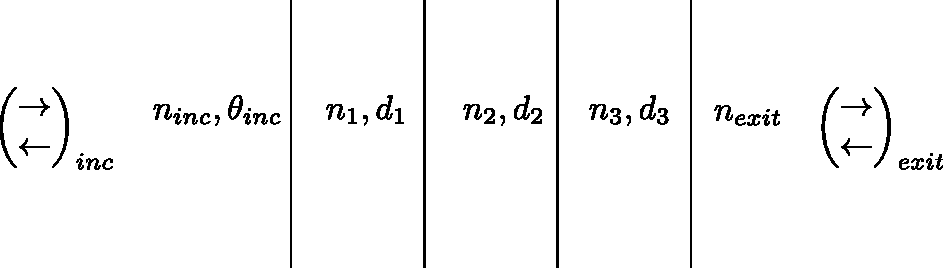
\includegraphics[height=3cm]{film.pdf}
\end{figure}
\paragraph{Polarisation perpendiculaire}

\begin{dmath}
\begin{pmatrix}\rightarrow \\ \leftarrow \end{pmatrix}_{inc} = 
\frac{1}{2 \eta_{inc}} \begin{pmatrix} \eta_{inc} & 1 \\ \eta_{inc} & -1 \end{pmatrix} \overbrace{ \begin{pmatrix} 1 & 1 \\ \eta_1 & -\eta_1 \end{pmatrix}
\begin{pmatrix} \psi_1^{-1} & 0 \\ 0 & \psi_1 \end{pmatrix}
\frac{1}{2 \eta_1} \begin{pmatrix} \eta_1 & 1 \\ \eta_1 & -1 \end{pmatrix} }^{L_1} \begin{pmatrix} 1 & 1 \\ \eta_2 & -\eta_2 \end{pmatrix}
\begin{pmatrix} \psi_2^{-1} & 0 \\ 0 & \psi_2 \end{pmatrix} \\
\frac{1}{2 \eta_2} \begin{pmatrix} \eta_2 & 1 \\ \eta_2 & -1 \end{pmatrix} \overbrace{ \begin{pmatrix} 1 & 1 \\ \eta_3 & -\eta_3 \end{pmatrix}
\begin{pmatrix} \psi_3^{-1} & 0 \\ 0 & \psi_3 \end{pmatrix}
\frac{1}{2 \eta_3} \begin{pmatrix} \eta_3 & 1 \\ \eta_3 & -1 \end{pmatrix} }^{L_3} \begin{pmatrix} 1 & 1 \\ \eta_{exit} & -\eta_{exit} \end{pmatrix}
\begin{pmatrix}\rightarrow \\ \leftarrow\end{pmatrix}_{exit} =
\frac{1}{2 \eta_{inc}} \begin{pmatrix} \eta_{inc} & 1 \\ \eta_{inc} & -1 \end{pmatrix} L_1 L_2 L_3 \begin{pmatrix} 1 & 1 \\ \eta_{exit} & -\eta_{exit} \end{pmatrix}
\begin{pmatrix}\rightarrow \\ \leftarrow\end{pmatrix}_{exit}
\end{dmath}

\begin{dmath}
L = \begin{pmatrix} 1 & 1 \\ \eta & -\eta \end{pmatrix} \begin{pmatrix} \psi^{-1} & 0 \\ 0 & \psi \end{pmatrix} \frac{1}{2 \eta} \begin{pmatrix} \eta & 1 \\ \eta & -1 \end{pmatrix} = 
\begin{pmatrix} \frac{\psi + \psi^{-1}}{2} & -\frac{\psi - \psi^{-1}}{2\eta} \\ -\eta\frac{\psi - \psi^{-1}}{2} & \frac{\psi + \psi^{-1}}{2} \end{pmatrix} =
\begin{pmatrix} \cos \delta & -\frac{i \sin \delta}{\eta} \\ -\eta i \sin \delta & \cos \delta \end{pmatrix}
\end{dmath}

où $\delta = n \frac{2\pi}{\lambda_0} d \cos \theta$

Si on prend $\begin{pmatrix}\rightarrow \\ \leftarrow\end{pmatrix}_{exit} = \begin{pmatrix}t \\ 0\end{pmatrix}$ et $\begin{pmatrix}\rightarrow \\ \leftarrow\end{pmatrix}_{inc} = \begin{pmatrix}1 \\ r\end{pmatrix}$ on a alors :
\begin{dmath}
\begin{pmatrix}1/t \\ r/t \end{pmatrix} = \frac{1}{2 \eta_{inc}} \begin{pmatrix} \eta_{inc} & 1 \\ \eta_{inc} & -1 \end{pmatrix} L_1 L_2 L_3 \begin{pmatrix} 1 \\ \eta_{exit} \end{pmatrix}
\end{dmath}


\paragraph{Polarisation parallèle}
\begin{dmath}
\begin{pmatrix}\rightarrow \\ \leftarrow \end{pmatrix}_{inc} = 
\frac{1}{2 n_{inc}} \begin{pmatrix} \eta_{inc} & 1 \\ \eta_{inc} & -1 \end{pmatrix} \overbrace{ \frac{n_1}{\eta_1} \begin{pmatrix} 1 & 1 \\ \eta_1 & -\eta_1 \end{pmatrix}
\begin{pmatrix} \psi_1^{-1} & 0 \\ 0 & \psi_1 \end{pmatrix}
\frac{1}{2 n_1} \begin{pmatrix} \eta_1 & 1 \\ \eta_1 & -1 \end{pmatrix} }^{L_1} \frac{n_2}{\eta_2} \begin{pmatrix} 1 & 1 \\ \eta_2 & -\eta_2 \end{pmatrix}
\begin{pmatrix} \psi_2^{-1} & 0 \\ 0 & \psi_2 \end{pmatrix} \\
\frac{1}{2 n_2} \begin{pmatrix} \eta_2 & 1 \\ \eta_2 & -1 \end{pmatrix} \overbrace{ \frac{n_3}{\eta_3} \begin{pmatrix} 1 & 1 \\ \eta_3 & -\eta_3 \end{pmatrix}
\begin{pmatrix} \psi_3^{-1} & 0 \\ 0 & \psi_3 \end{pmatrix}
\frac{1}{2 n_3} \begin{pmatrix} \eta_3 & 1 \\ \eta_3 & -1 \end{pmatrix} }^{L_3} \frac{n_{exit}}{\eta_{exit}} \begin{pmatrix} 1 & 1 \\ \eta_{exit} & -\eta_{exit} \end{pmatrix}
\begin{pmatrix}\rightarrow \\ \leftarrow\end{pmatrix}_{exit} =
\frac{1}{2 n_{inc}} \begin{pmatrix} \eta_{inc} & 1 \\ \eta_{inc} & -1 \end{pmatrix} L_1 L_2 L_3 \frac{n_{exit}}{\eta_{exit}} \begin{pmatrix} 1 & 1 \\ \eta_{exit} & -\eta_{exit} \end{pmatrix}
\begin{pmatrix}\rightarrow \\ \leftarrow\end{pmatrix}_{exit}
\end{dmath}

Les matrices $L$ ont la même forme que dans le cas perpendiculaire.

Si on prend $\begin{pmatrix}\rightarrow \\ \leftarrow\end{pmatrix}_{exit} = \begin{pmatrix}t \\ 0\end{pmatrix}$ et $\begin{pmatrix}\rightarrow \\ \leftarrow\end{pmatrix}_{inc} = \begin{pmatrix}1 \\ r\end{pmatrix}$ on obtient :
\begin{dmath}
\begin{pmatrix}1/t \\ r/t \end{pmatrix} = \frac{1}{2 n_{inc}} \begin{pmatrix} \eta_{inc} & 1 \\ \eta_{inc} & -1 \end{pmatrix} L_1 L_2 L_3 \frac{n_{exit}}{\eta_{exit}} \begin{pmatrix} 1 \\ \eta_{exit} \end{pmatrix}
\end{dmath}

On peut écrire différemment le terme suivant :
\begin{dmath}
\frac{1}{n_{inc}} \frac{n_{exit}}{\eta_{exit}} = \frac{1}{\eta_{inc} \cos \theta_{inc}} \frac{n_{exit}}{n_{exit} / \cos \theta_{exit}}
= \frac{1}{\eta_{inc}} \frac{\cos \theta_{exit}}{\cos \theta_{inc}}
\end{dmath}

Pour avoir au final :
\begin{dmath}
\begin{pmatrix}1/t \\ r/t \end{pmatrix} = \frac{\cos \theta_{exit}}{\cos \theta_{inc}} \frac{1}{2 \eta_{inc}} \begin{pmatrix} \eta_{inc} & 1 \\ \eta_{inc} & -1 \end{pmatrix} L_1 L_2 L_3 \begin{pmatrix} 1 \\ \eta_{exit} \end{pmatrix}
\end{dmath}














\section{Coefficients de transmition et reflexion}
\paragraph{Polarisation perpendiculaire}

\begin{dmath}
\begin{pmatrix}1/t \\ r/t \end{pmatrix} = \frac{1}{2 \eta_{inc}} \begin{pmatrix} \eta_{inc} & 1 \\ \eta_{inc} & -1 \end{pmatrix} L_1 L_2 L_3 \begin{pmatrix} 1 \\ \eta_{exit} \end{pmatrix}
\end{dmath}

Si on définit
\begin{dmath}
\begin{pmatrix} b \\ c \end{pmatrix} = L_1 L_2 L_3 \begin{pmatrix} 1 \\ \eta_{exit} \end{pmatrix}
\end{dmath}


\begin{dmath}
\begin{pmatrix}1/t \\ r/t \end{pmatrix} = \begin{pmatrix} \frac{b + c / \eta_{inc}}{2} \\ \frac{b - c / \eta_{inc}}{2} \end{pmatrix} \Rightarrow
\left\{ \begin{array}{l}
	t = \frac{2}{b + c / \eta_{inc}} \\
	r = \frac{b - c / \eta_{inc}}{2} \frac{2}{b + c / \eta_{inc}} = \frac{b - c / \eta_{inc}}{b + c / \eta_{inc}}
\end{array} \right.
\end{dmath}


\paragraph{Polarisation parallèle}
\begin{dmath}
\begin{pmatrix}1/t \\ r/t \end{pmatrix} = \frac{\cos \theta_{exit}}{\cos \theta_{inc}} \frac{1}{2 \eta_{inc}} \begin{pmatrix} \eta_{inc} & 1 \\ \eta_{inc} & -1 \end{pmatrix} L_1 L_2 L_3 \begin{pmatrix} 1 \\ \eta_{exit} \end{pmatrix}
\end{dmath}

\begin{dmath}
\begin{pmatrix}1/t \\ r/t \end{pmatrix} =  \frac{\cos \theta_{exit}}{\cos \theta_{inc}} \begin{pmatrix} \frac{b + c / \eta_{inc}}{2} \\ \frac{b - c / \eta_{inc}}{2} \end{pmatrix} \Rightarrow
\left\{ \begin{array}{l}
	t = \frac{2}{b + c / \eta_{inc}} \frac{\cos \theta_{inc}}{\cos \theta_{exit}} \\
	r = \frac{b - c / \eta_{inc}}{b + c / \eta_{inc}}
\end{array} \right.
\end{dmath}

\end{document}
